\documentclass{beamer}
\usetheme{Madrid}

\usepackage{pgfplots}

\title{Stochastic Gradient Descent}
\subtitle{STAT 672 Project}
\author{Tom Wallace}
\institute{George Mason University}
\date{Spring 2018}



\AtBeginSection[]{
\begin{frame}
\frametitle{Table of Contents}
\tableofcontents[currentsection]
\end{frame}
}

\begin{document}

\frame{\titlepage}

%%%%%%%%%%%%% Introduction %%%%%%%%%%%%%%
\begin{frame}

\frametitle{Introduction}
\textbf{Stochastic gradient descent (SGD)} is an optimization algorithm that is
fundamental to many machine learning approaches. We will examine SGD from four
perspectives. 

\tableofcontents

\end{frame}

\section{Motivation}
\begin{frame}
\frametitle{Optimization is everywhere, and sometimes easy}
Many statistical procedures involve minimizing or maximizing some function 
applied to data \\~\\

In \textbf{parametric} statistics, we often make assumptions about the
distribution of the data that make this optimization ``nice'' (convex or
concave) \\~\\

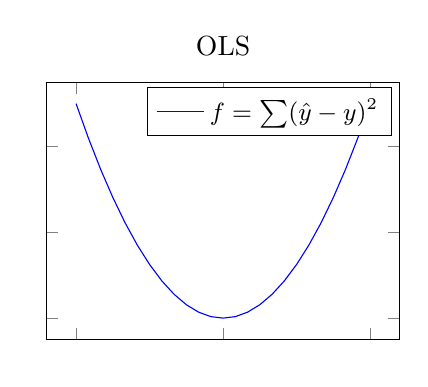
\begin{tikzpicture}
\begin{axis}[
title={OLS},
yticklabels={,,},
xticklabels={,,},
width=0.5\textwidth,
height=0.4\textwidth,
legend style = {font=\small}
]
\addlegendentry{$f=\sum (\hat{y} - y)^2$}
\addplot[mark=none, color=blue]{x^2};
\end{axis}
\end{tikzpicture}
\hskip 5pt
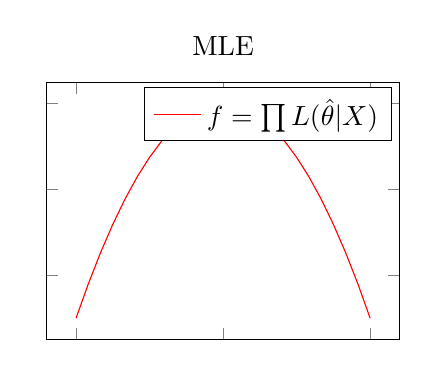
\begin{tikzpicture}
\begin{axis}[
title={MLE},
yticklabels={,,},
xticklabels={,,},
width=0.5\textwidth,
height=0.4\textwidth
]
\addlegendentry{$f=\prod L(\hat{\theta} | X)$}
\addplot[mark=none, color=red]{-(x^2)};
\end{axis}
\end{tikzpicture}
\end{frame}

\begin{frame}
\frametitle{Other times, optimization is not easy}
In \textbf{non-parametric} settings, we conduct \textbf{empirical risk
minimization}
\end{frame}

\section{Mathematical Foundations}
\begin{frame}
foo
\end{frame}

\section{Implementation}
\begin{frame}
foo
\end{frame}

\section{Real-World Usage}
\begin{frame}
foo
\end{frame}
\end{document}


